\section{Results \& Discussion}\label{sec:results}

%\begin{itemize}
%	\item Describe your results in a clrear and understandable way.
%	\item Clearly differentiate between what you have achieved and what you have build upon.
%	\item Ideally add some sort of visual representation of your result that underlines the progress you have made during the research project.
%	\item Make sure that the results are reproducible by your reader if needed
%	\item Critically discuss your results.
%	\item Did you achieve what you set out to do?
%	\item What are the strengths and weaknesses of your research?
%\end{itemize}
In this section, we discuss our dataset, evaluate our machine learning model and present our final mobile application.
\subsection{Dataset}
The training dataset consists of 116 samples with 49 female and 67 male swimmers. The test dataset contains 19 samples, ten of which are female. The swimming times in the dataset were achieved at the same competition on the same weekend in a 25m pool. Both datasets cover ages from nine to 14 years and training ages from one to seven years.
\begin{figure}[ht]
    \centering
    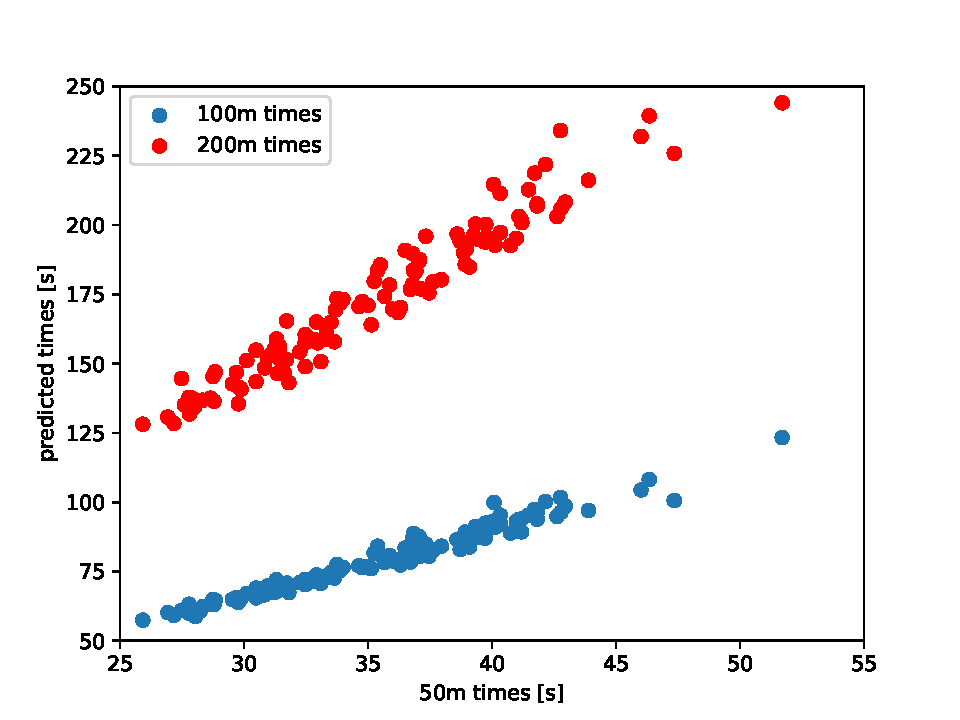
\includegraphics[scale=0.5]{visualisation/training_data.pdf}
    \caption{Training data: correlation of 50m and longer distance times}
    \label{fig:training_data}
\end{figure}
Figures \ref{fig:training_data} and \ref{fig:test_data} show the correlation of 50m and the longer distance times. In order to plot the samples in 2D, we omit the information about the swimmer. We can see that the times have a strong linear correlation with a Pearson correlation coefficient of $0.983$ for the 100m training data and $0.972$ for the 200m training data. Therefore, our initial assumption that age is essential for the prediction was wrong. Even for junior swimmers, the times follow a linear correlation as introduced by the critical power concept in section \ref{critical_power}, independent of the age, the training age or the gender.\\
\begin{figure}[ht]
    \centering
    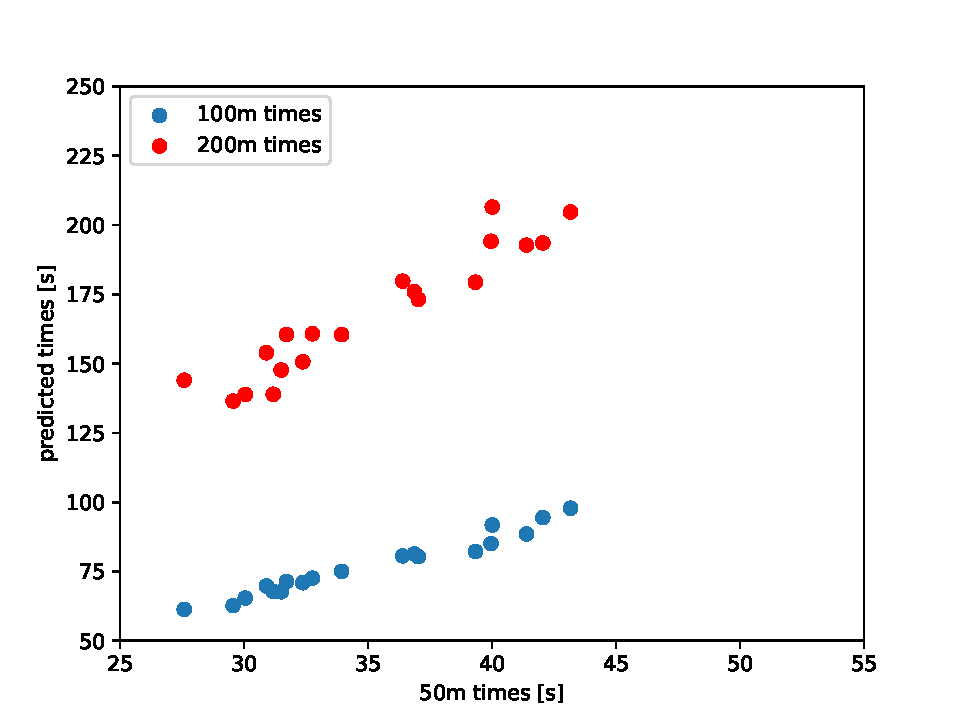
\includegraphics[scale=0.5]{visualisation/test_data.pdf}
    \caption{Test data: correlation of 50m and longer distance times}
    \label{fig:test_data}
\end{figure}
Also, we observe a higher variance in the long-distance times for higher 50m times. As we can see in Figure \ref{fig:training_age}, these higher 50m times are mostly from swimmers that are in their first or second training year. These swimmers have less competition experience or a rather bad technique. Moreover, young swimmers are often very nervous at competitions; thus, they make mistakes more likely. This makes it harder to predict their performance. The better a swimmer is, i.e. the longer he trains and the better his technique is, the more reliable his performance will be.
\begin{figure}[ht]
    \centering
    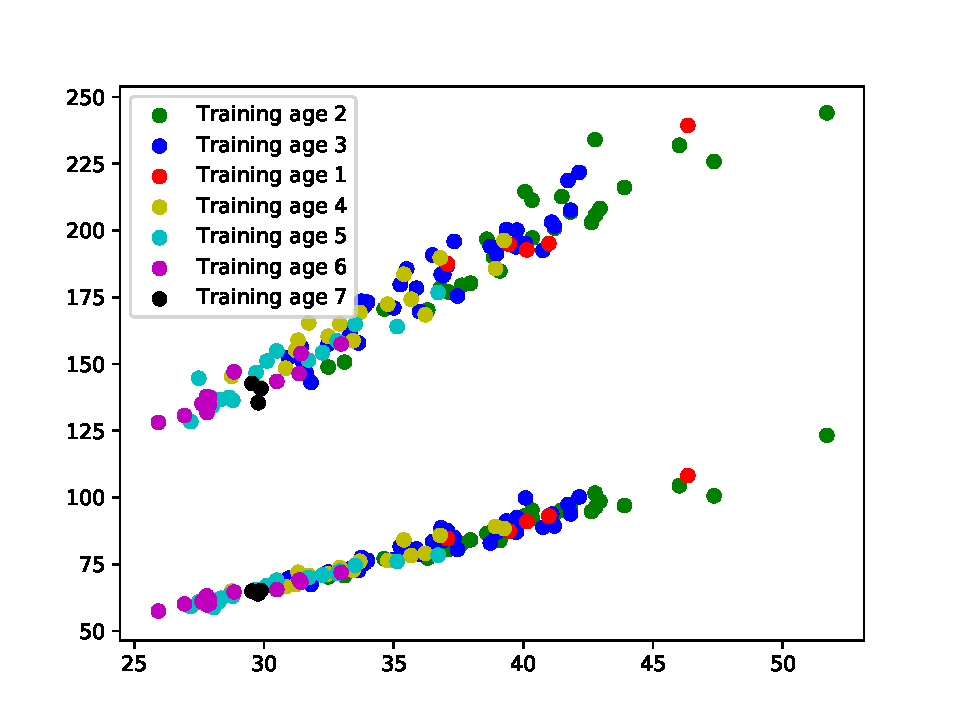
\includegraphics[scale=0.5]{visualisation/training_data_train_ages.pdf}
    \caption{Training data: influence of training age}
    \label{fig:training_age}
\end{figure}
\subsection{Model selection}
\begin{centering}
\begin{tabular}{|cc|c|c|c|}\hline
    &&\multicolumn{3}{c|}{\textbf{Units}}\\
    & & 16 & 32 & 64 \\\hline
    \multirow{2}{*}{\textbf{rmsprop}}&100m&1.94&1.90&1.97\\\cline{2-5}
    &200m&5.35&5.49&5.92\\\hline
    \multirow{2}{*}{\textbf{adam}}&100m&4.88&5.28&2.48\\\cline{2-5}
    &200m&10.40&8.55&8.47\\\hline
\end{tabular}
\captionof{table}{Mean absolute error for different units in input layer}
\label{tab:hyperparam_units}
\end{centering}
As we have seen in the previous section, the data is linearly separable; thus, we do not need a hidden layer in our model. In the next step, we need to find the units for the Dense input layer as well as the best optimiser for our model. Therefore, we train models using $\{16, 32, 64\}$ neurons and Adam or RMSprop as optimiser. The models are trained using the training data and tested against the validation data. The results are presented in Table \ref{tab:hyperparam_units}.\\
We can see that RMSprop is the best optimiser; thus, we use RMSprop with 32 units for the 100m prediction and RMSprop with 16 units for the 200m prediction.
\subsection{Model evaluation}
\begin{figure*}[ht]
\begin{minipage}{0.62\textwidth}
\begin{tabular}{|c|c|c|c|}\hline
    Model &Training data&Test data&Error  \\\hline
    \makecell{
\includegraphics[scale=0.5]{visualisation/blue_square.png}\\original}&swimmer info, 50m&swimmer info, 50m&7.97\\\hline
    
\includegraphics[scale=0.5]{visualisation/yellow_circle.png}&\makecell{swimmer info, 50m,\\ true 100m}& \makecell{swimmer info, 50m,\\ true 100m}&5.77\\\hline
    
\includegraphics[scale=0.5]{visualisation/red_circle.png}&\makecell{swimmer info, 50m,\\ true 100m}&\makecell{swimmer info, 50m,\\ predicted 100m}&8.30\\\hline
    
\includegraphics[scale=0.5]{visualisation/green_triangle.png}&\makecell{swimmer info, 50m,\\ predicted 100m}&\makecell{swimmer info, 50m,\\ predicted 100m}&7.67\\\hline
\end{tabular}
\end{minipage}
\begin{minipage}{0.38\textwidth}
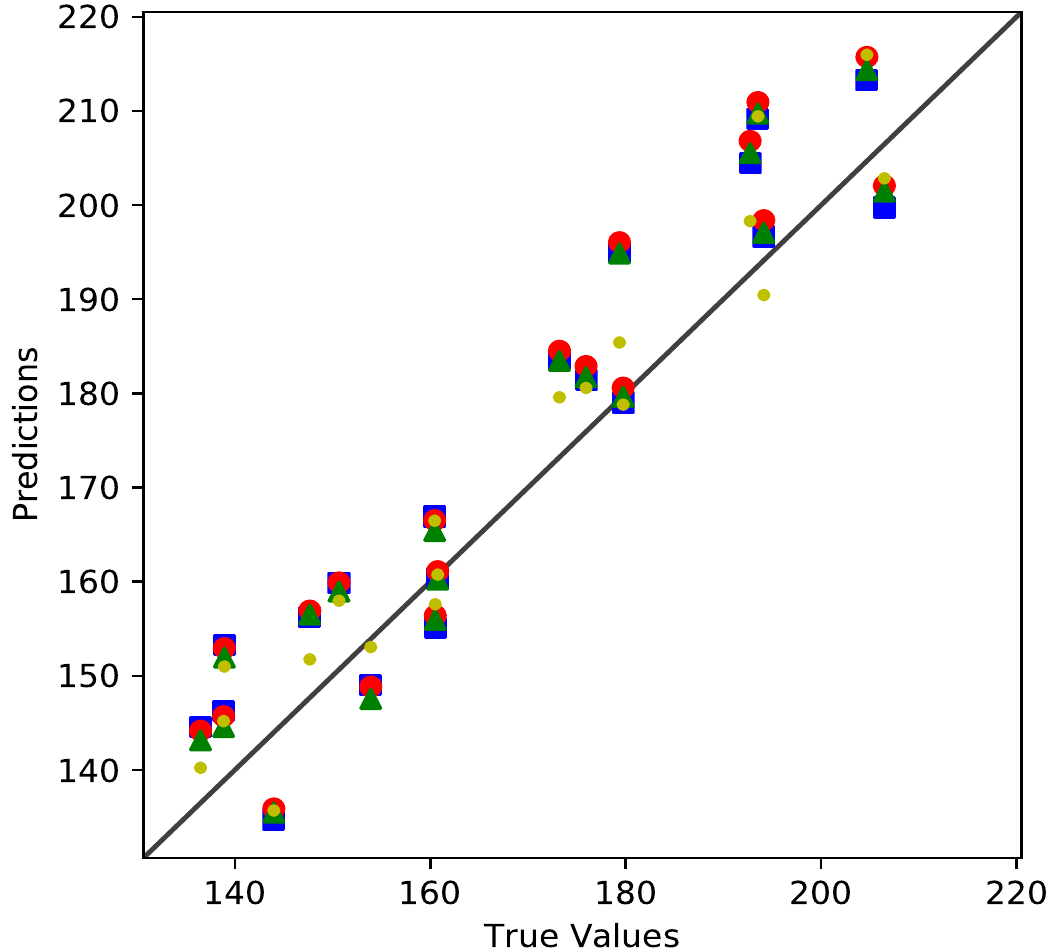
\includegraphics[width=\textwidth]{visualisation/eval_200m_variations.png}
\end{minipage}
\caption{Comparison of different 200m approaches}
\label{fig:200m_variations}
\end{figure*}
We evaluate the model using the test dataset. Figure 7 shows the scatter of the predicted and the correct 100m times as well as the predicted and correct 200m times. The black line in each plot represents the optimum, where predicted and correct times are identical thus the closer the dots are to this line, the better is the model.\\
\begin{figure}[ht]
    \begin{minipage}{0.23\textwidth}
    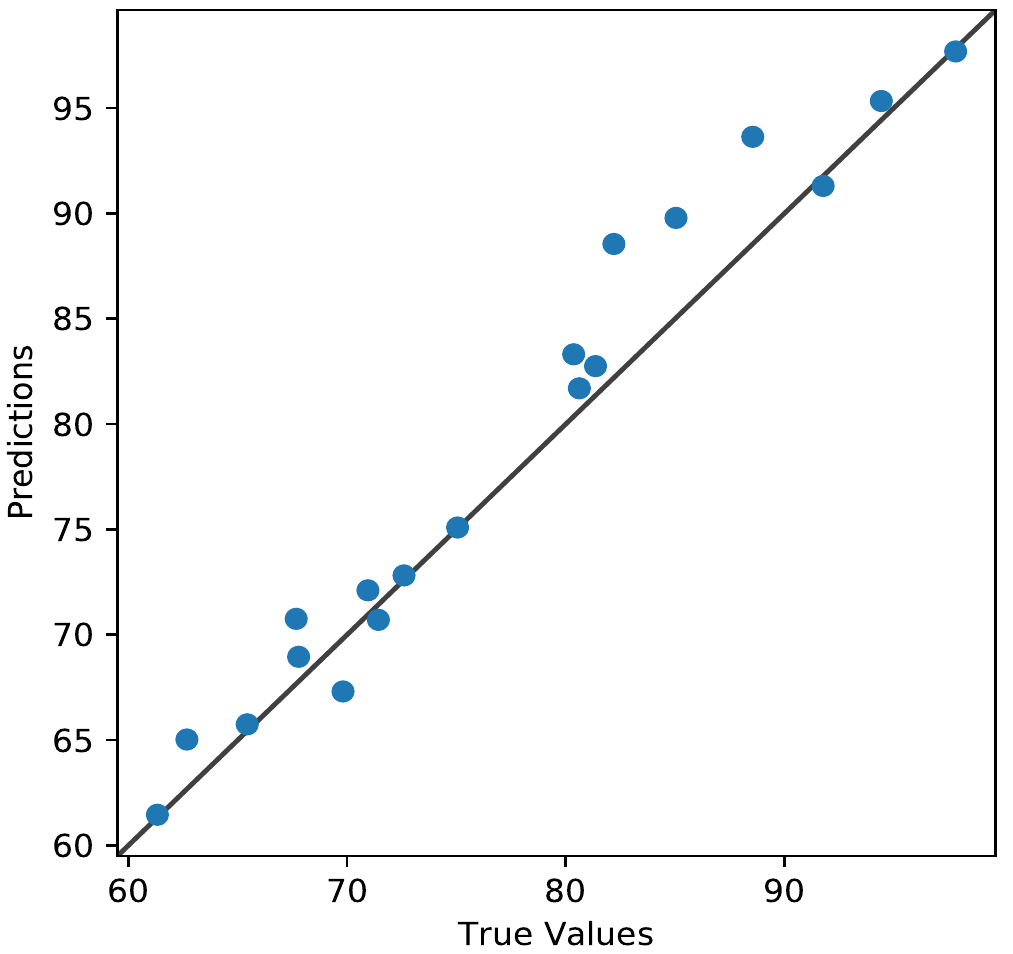
\includegraphics[width=\textwidth]{visualisation/eval_100m.png}
\end{minipage}
\begin{minipage}{0.23\textwidth}
    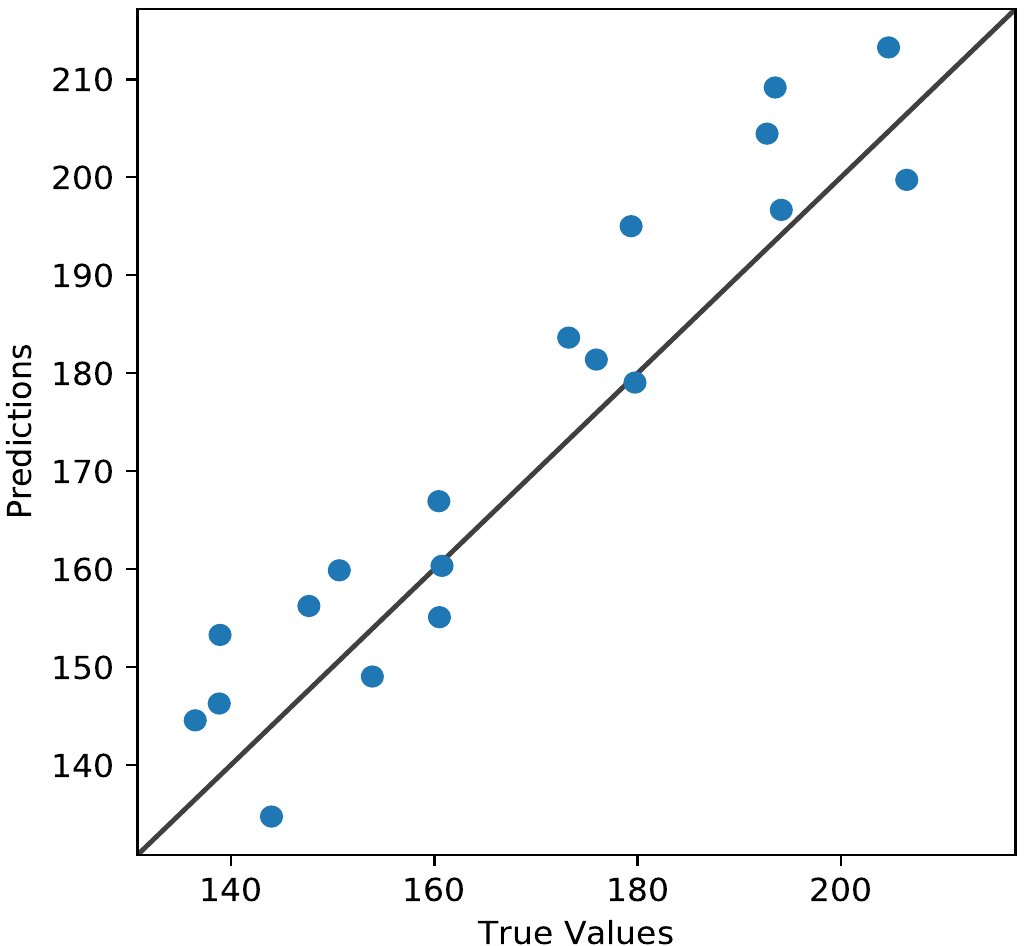
\includegraphics[width=\textwidth]{visualisation/eval_200m.png}
\end{minipage}
\caption{Evaluation of 100m (left) and 200m (right) model}
\label{fig:eval_model}
\end{figure}
The models achieve a mean-absolute error of $1.83$ for the 100m model and $7.97$ for the 200m model. We consider the 100m prediction as successful thus we use this model in our application.\\
The 200m prediction, however, has deficits. A potential improvement could be to include the 100m times in the 200m prediction. In order to evaluate this idea, we train two additional models. For the first model, we add the correct 100m times to the training data and for the second model, we use the 100m model to predict the 100m times and add these times to the training data. Figure \ref{fig:200m_variations} evaluates the four resulting models. The small yellow circles use the correct 100m times for training and prediction. It is important to mention that this model is only for theoretical analysis and does not apply to our real-world problem as we do not know the correct 100m times when we predict new samples. However, this model shows that using the 100m times for the 200m prediction can indeed improve the results. The models using the predicted 100m times for the 200m prediction do not perform better than the original model. Moreover, we can see in the plot that these models almost ignore the 100m time as their predicted times are nearly identical. A reason for this is that the 100m prediction model is not good enough to be helpful for the 200m prediction. Finally, using the 100m times for the 200m model is a good idea but does not work in practice; thus, we use the original 200m model in our application.
\subsection{Android application}
Figure \ref{fig:app_screenshots} shows screenshots of the final Android application. 

In this section, we highlight the interesting implementation considerations of the Android application. We explain the stopwatch logic in Figure \ref{fig:stopwatch_logic}. At first the stopwatch is set to zero. When the play button is clicked, the time starts to run and the play icon on the play/pause button changes to a pause icon. When clicking the pause button, the stopwatch stops running, displays the current time and the button shows the play icon again. The time is saved into a shared preference object and loaded into the 50m time field of the prediction view thus the user does not need to transfer the time himself. The stopwatch can be reset at any time. If the reset button is clicked, the displayed time and the time stored in the shared preferences are set to zero again. We simulate the running stopwatch using a java $Runnable$ object that displays the difference between the start time and the current system time \footnote{\url{https://www.android-examples.com/android-create-stopwatch-example-\ tutorial-in-android-studio/}, accessed 31.12.2019}.\\
\begin{figure}[ht]
    \centering
    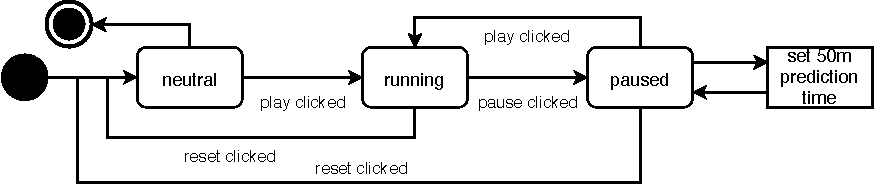
\includegraphics[scale=0.5]{visualisation/StopwatchLogic.pdf}
    \caption{Activity diagram for stopwatch function}
    \label{fig:stopwatch_logic}
\end{figure}
\begin{figure}[ht]
\centering
\begin{minipage}{0.2\textwidth}
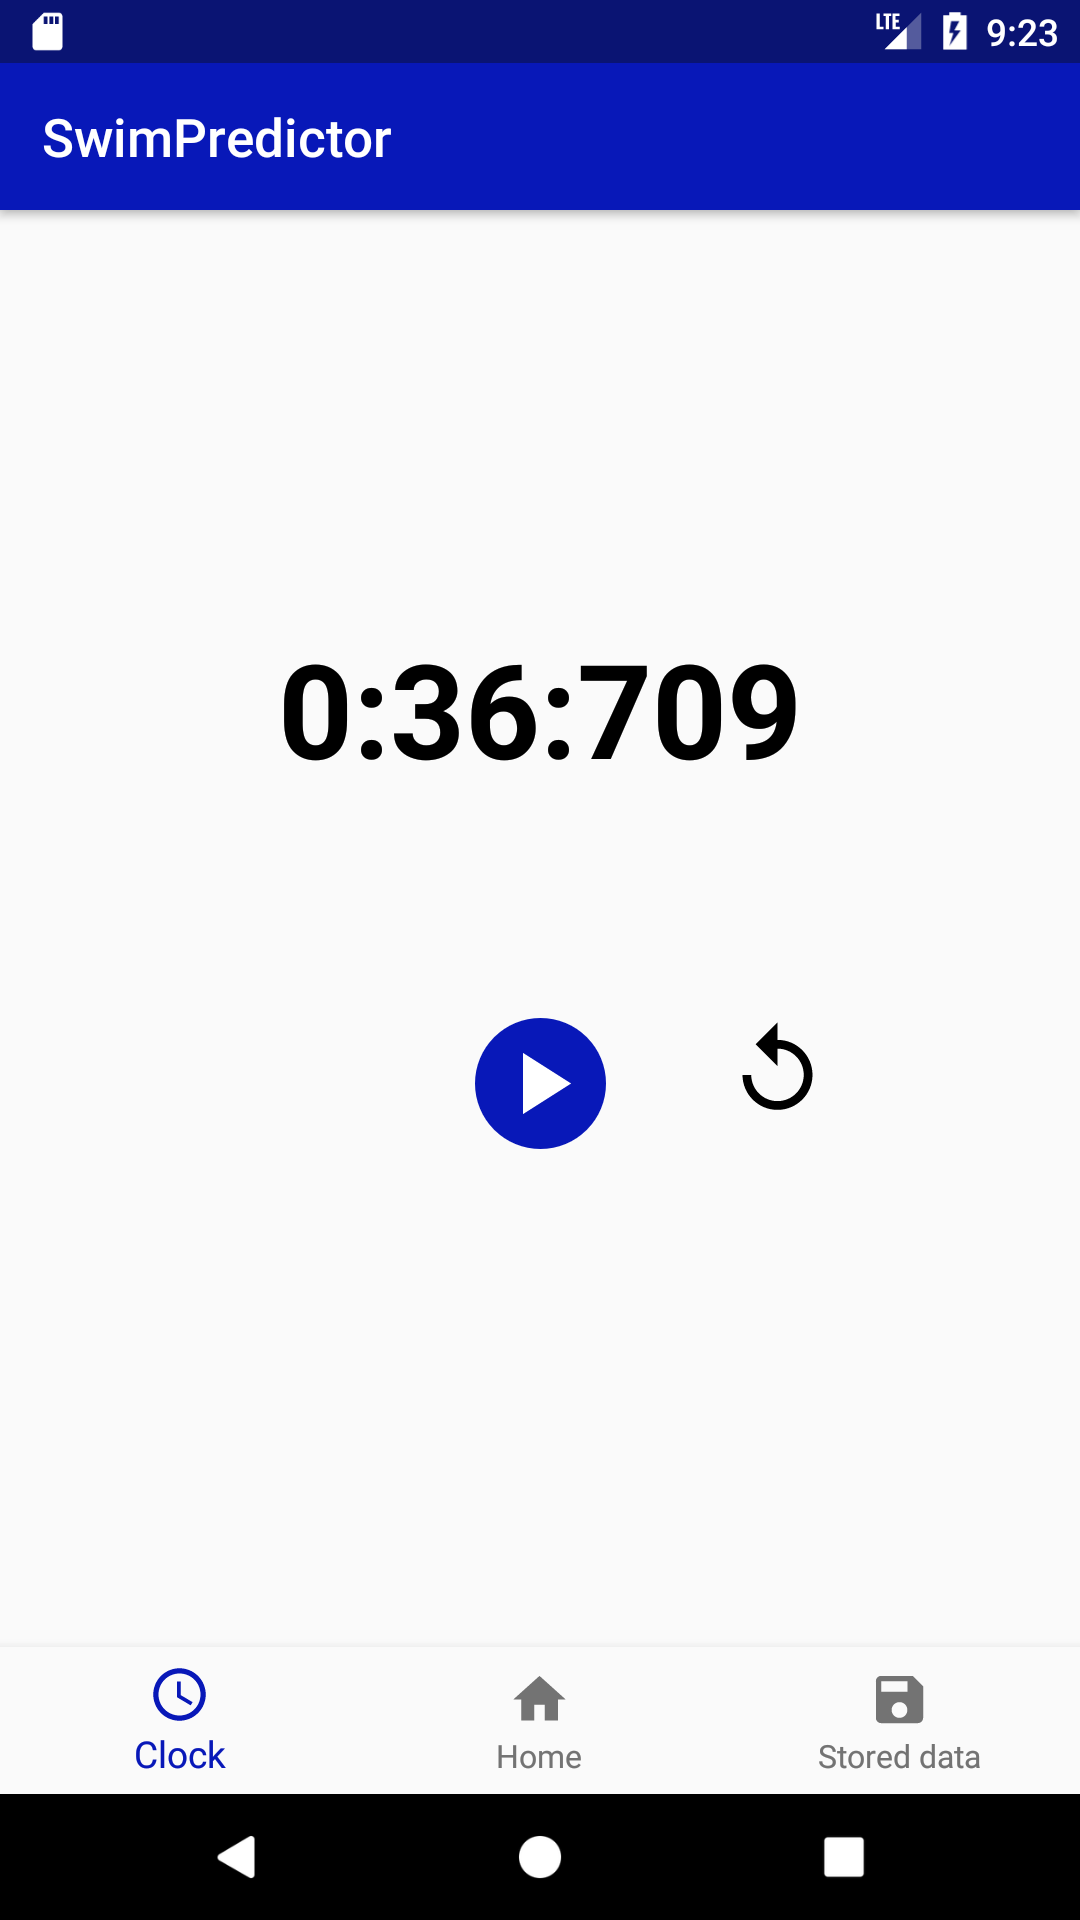
\includegraphics[width=\textwidth]{visualisation/stopwatch_view.png}
\end{minipage}
\begin{minipage}{0.2\textwidth}
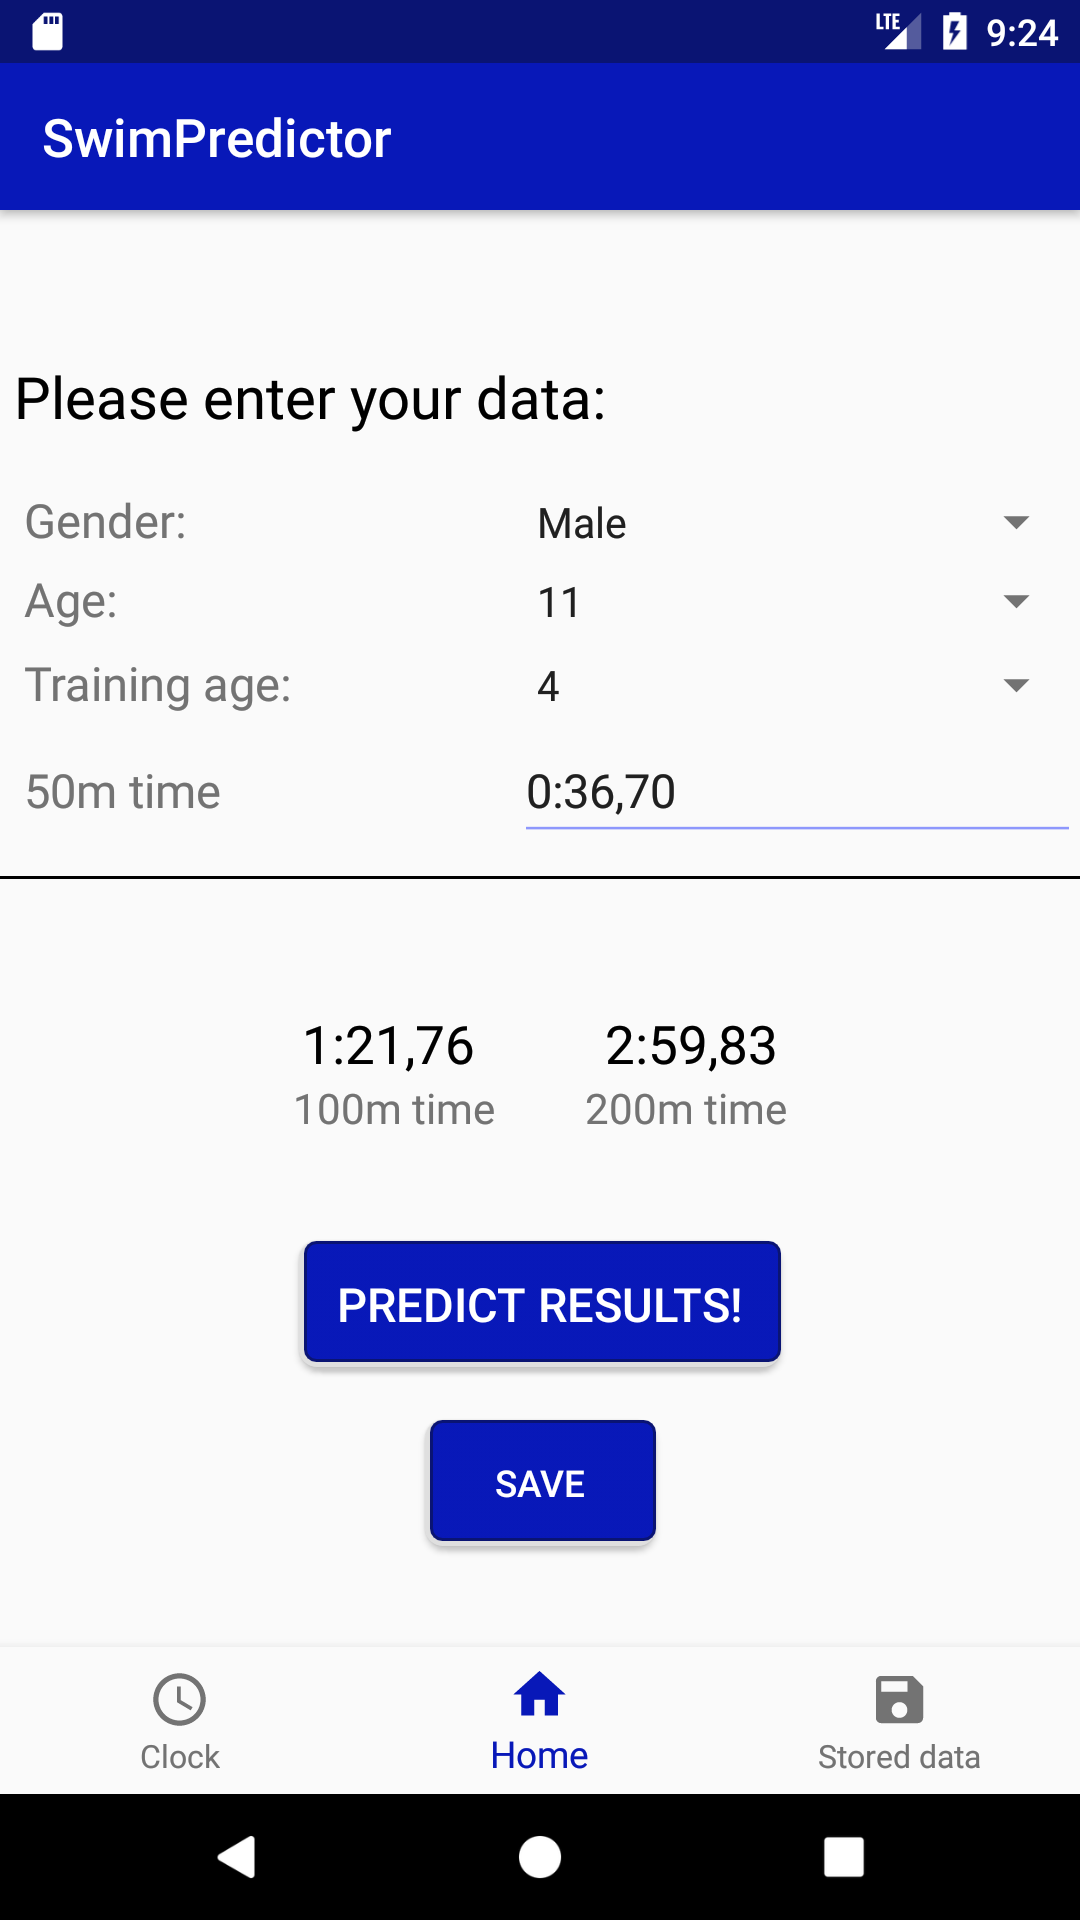
\includegraphics[width=\textwidth]{visualisation/prediction_view.png}
\end{minipage}
\caption{Screenshots of the app's stopwatch and home view}
\label{fig:app_screenshots}
\end{figure}
The database behind our app contains one table. A \texttt{DataSample} object represents an entity in this table and contains all the information from the data records, as explained in section \ref{sec:data_gen}, together with a unique description that the coach enters when saving a record and human-readable String representation of the times. These Strings have the format \texttt{m:ss,dscs}, e.g. \texttt{1:23,45}.\\
We had problems to display the entries in the database as the number of entries in the database changes thus a static TableView is not applicable. Therefore, we use the Open-Source version of the SortableTableView\footnote{\url{https://github.com/ISchwarz23/SortableTableView}, accessed 12.01.2020}. Due to the small display on a mobile device, we were not able to show all information of all samples at the same time. Therefore, the table only shows the description and the three times. The remaining information about the swimmer can be shown in a pop- up message when clicking at the respective sample. To delete a sample, the user needs to long click on the sample he wants to delete. The app then requires a confirmation of the user. If he confirms the deletion, the sample is removed from the database, and the table is reloaded. Figure \ref{fig:app_screenshots_database} shows the TableView of the database entries as well as the pop-up messages with detailed information and deletion confirmation.
\begin{figure}[ht]
\begin{minipage}{0.15\textwidth}
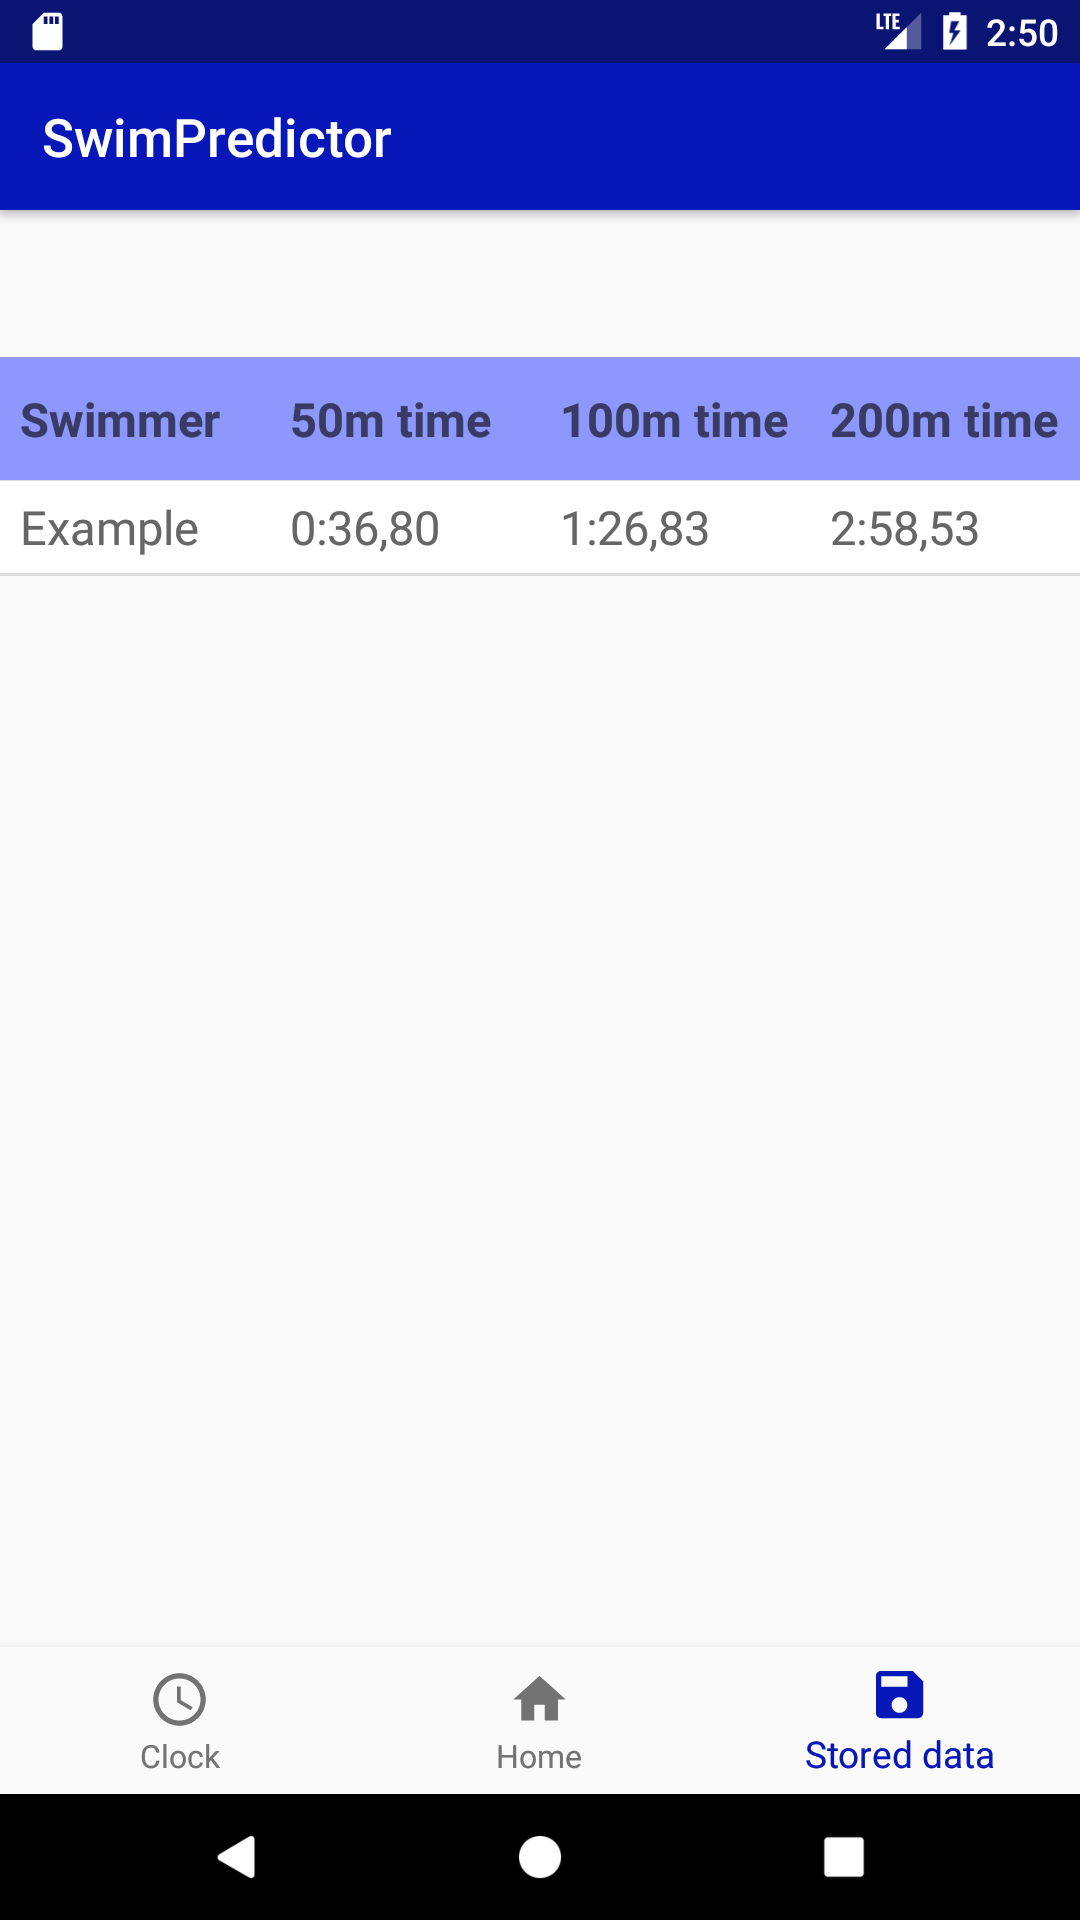
\includegraphics[width=\textwidth]{visualisation/database_view.png}
\end{minipage}
\begin{minipage}{0.15\textwidth}
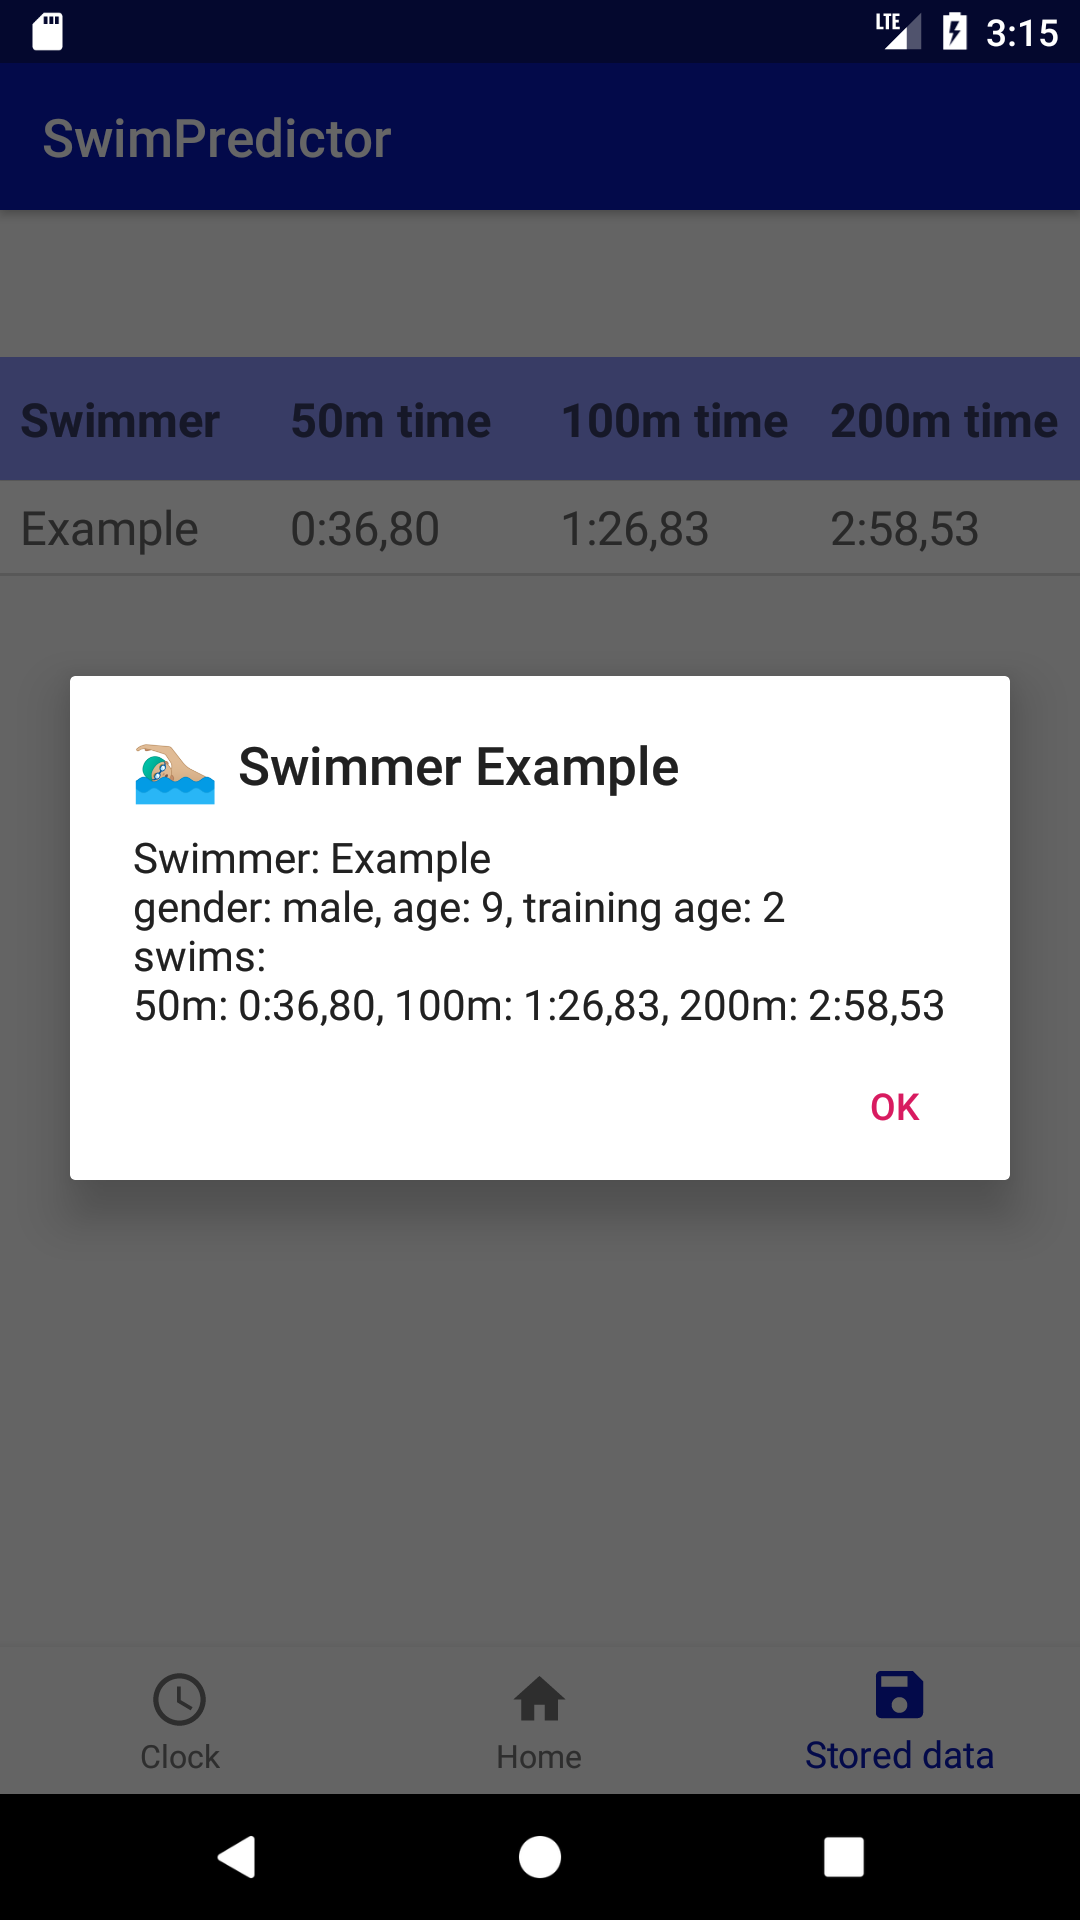
\includegraphics[width=\textwidth]{visualisation/app_detailed_information.png}
\end{minipage}
\begin{minipage}{0.15\textwidth}
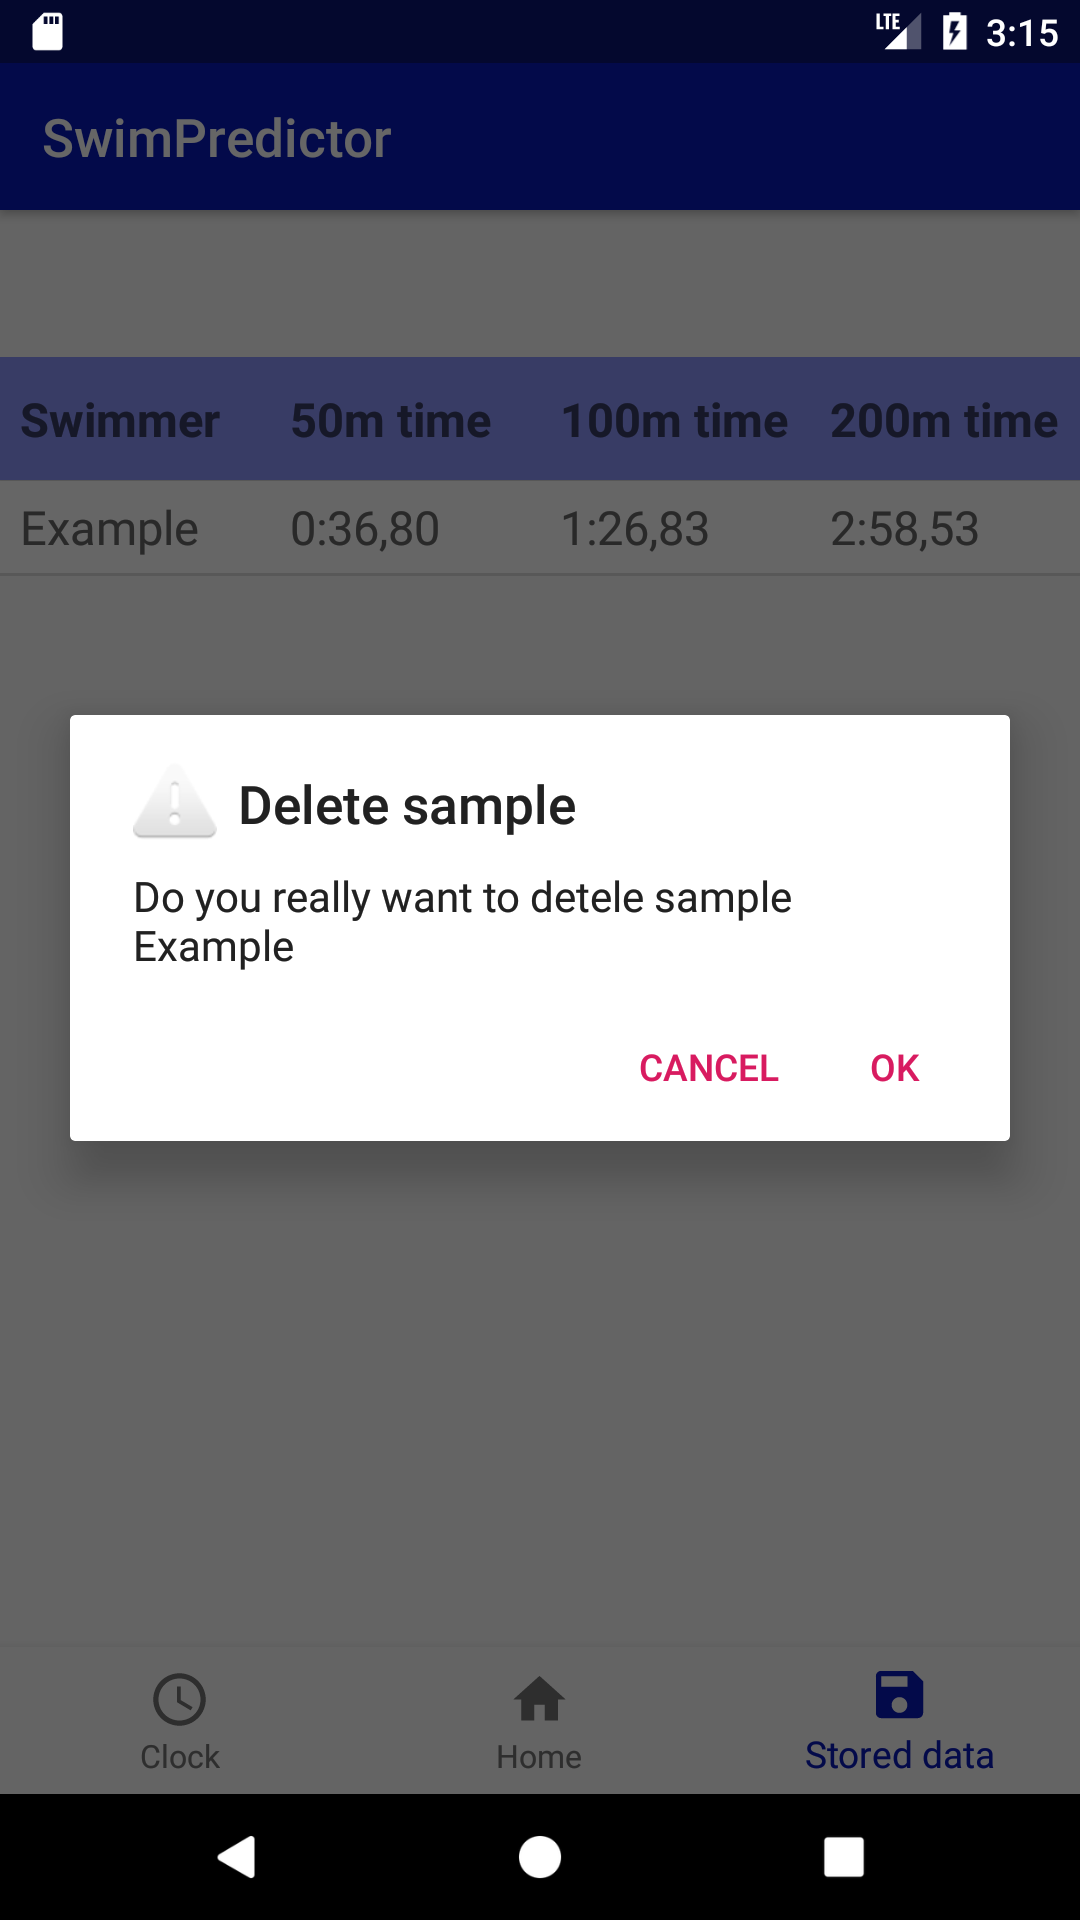
\includegraphics[width=\textwidth]{visualisation/app_confirm_deletion.png}
\end{minipage}
\caption{Screenshots of the app's database functionality}
\label{fig:app_screenshots_database}
\end{figure}